\section{Handlebodies}
\label{section:problem-handlebodies}

Handlebodies are objects central to arguments found near the end of Chapters \ref{chapter:smooth} and \ref{chapter:triangulation}.
A handlebody is formed by attaching some number of $(n,\lambda)$--handles to an $(n,0)$--handle.
The name is evoked by the type of handlebody that we examine in this section: the (3,1)--handlebody.

\begin{defn}
	A connected $n$--manifold $M$ that has a handle decomposition consisting of exactly one 0--handle and $g$ $\lambda$--handles is called an \emph{$(n,\lambda)$--handlebody} of \emph{genus} $g$.
	
	Let $V$ be an $(n,1)$--handlebody of genus $g$.
	A simple closed curve in $\pd V$ is called \emph{essential} if it is not homotopic to a point.
	A simple closed curve $J$ in $\pd V$ that is essential in $\pd V$ and that bounds a 2--disc in $V$ is called a \emph{meridian}.
	The properly embedded disc in $V$ that has boundary $J$ is called a \emph{meridinal disc}.
	
	The special case of the oriented genus 1 $(m,1)$--handlebody is called a \emph{solid torus}.
	More generally, any space that is homeomorphic to $S^1\times D^{n-1}$ is called a \emph{solid $n$--torus}.
	In our most common case of $n=3$, we just say that $S^1\times D^2$ is a \emph{solid torus}.
	A simple closed curve $J$ in the boundary of a solid torus that intersects a meridian at a single point is called a \emph{longitude}.
	A longitude is essential in a solid torus and there are infinitely many isotopy classes of longitudes, but there is exactly one isotopy class of meridians.
\end{defn}

We apply handlebodies to 3--manifold classification through Heegaard splittings.
%When you build a 3--manifold by gluing a pair of genus $g$ (3,1)--handlebodies together over their boundaries, you have formed a Heegaard splitting.

\begin{defn}	
	Let $U$ and $V$ be 3--dimensional handlebodies of genus $g$ and let $f:\pd U\to \pd V$ be an orientation preserving diffeomorphism.
	The adjunction $M=U\cup_f V$ is a \emph{Heegaard splitting} of $M$, the shared boundary $H = \pd U = \pd V$ is the \emph{Heegaard surface} of the splitting, and the shared genus of $U$ and $V$ is the \emph{genus} of the splitting as well.
	A Heegaard splitting is also denoted by the pair $(M,H)$.
	
	We use the notion of equivalence between splittings from \cite{SchlWald}:
	A pair of splittings $(M,H)$ and $(M,H')$ are \emph{equivalent} if there is a homeomorphism $h:M\to M$ such that $h$ is isotopic to $\texttt{id}M$ and $h|_H$ is an orientation preserving homeomorphism $H\to H'$.
\end{defn}

\begin{figure}[h!]
	\centering
	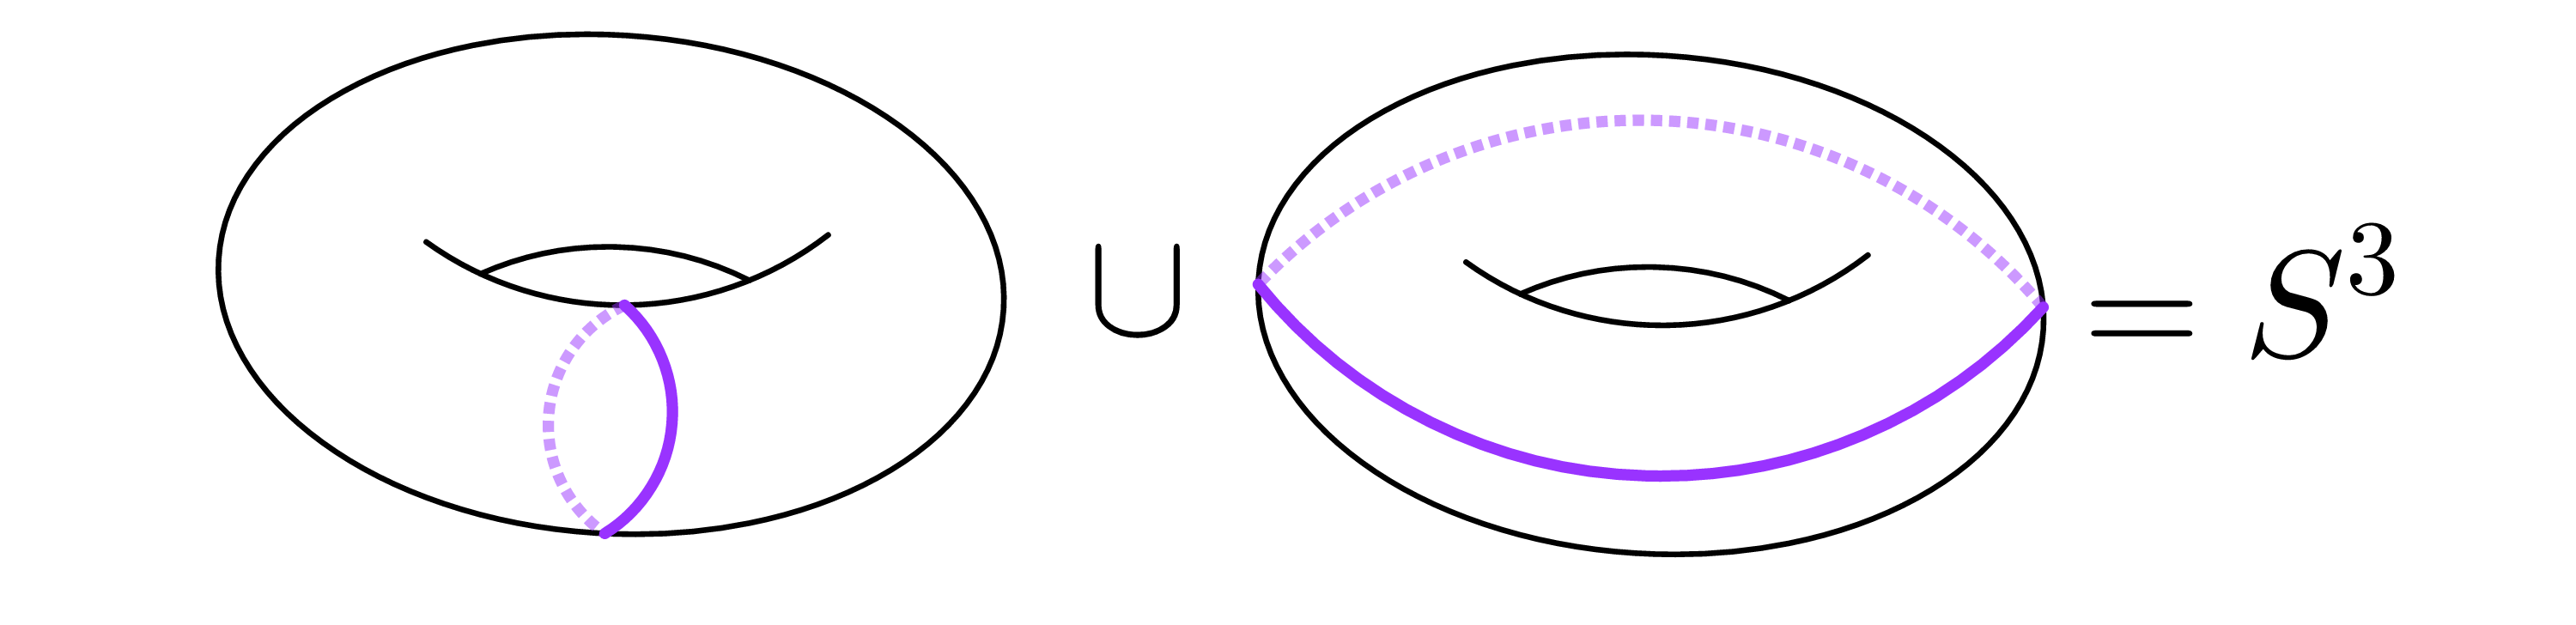
\includegraphics[width=\textwidth]{figures/genus-1-split.png}
	\caption{
		\textbf{Genus 1 Heegaard splitting of $S^3$.}
		The purple curve is essential in each solid torus pictured.
		In the left torus it is a meridian, on the right a longitude.
	}
	\label{fig:genus-1-split}
\end{figure}

\begin{ex}
	The 3--sphere $S^3$ has two standard Heegaard splittings.
	The first is the genus 0 splitting, which is realized by considering $S^3$ as the set of unit vectors in $\R^4$.
	Take the Heegaard surface to be the intersection of $S^3$ with the $xyz$--hyperplane in $\R^4$.
	This is a copy of $S^2$ that separates $S^3$ into two connected components.
	This splitting is written $(S^3,S^2)$
	
	The second is the genus 1 splitting, which is visualized using the realization of $S^3$ as the one--point compactification of $\R^3$.
	Take solid tori $U$ and $V$ and identify $\pd U$ with $\pd V$ by the homeomorphism that swaps a meridian with a longitude.
	The adjunction is $S^3$, and this splitting is written $(S^3,T^2)$.
	Figure \ref{fig:genus-1-split} displays the tori of the splitting.
	This description of $S^3$ is also obtained by examining the boundary of a 4--dimensional 2--handle $\pd (D^2\times D^2)$.
\end{ex}

\begin{defn}
	Let $(M,H)=U\cup_f V$ be a Heegaard splitting of $M$.
	The connected sum $(M,H)\#(S^3,T^2)$ is called an \emph{elementary stabilization} of $M$, and itself is a splitting $(M,H\#T^2)$.
	A Heegaard splitting $(M,H)$ is called a \emph{stabilization} of another splitting $(M,H')$ if it obtained from $(M,H')$ via a finite number of elementary stabilizations.
\end{defn}

Consider the meridians of the solid tori in the standard genus 1 splitting of $S^3$.
They each bound a disc in their respective handlebody, and they intersect in exactly one point.
We would expect to be able to find such curves in any 3--manifold obtained as a stabilization.

\begin{defn}	
	Let $(M,H)=U\cup_f V$ be a Heegaard splitting of genus $g$ and let $\alpha$, $\beta$ a pair of simple, closed, essential curves in $H$.
	Let $\alpha$ be a meridian of $U$ and $\beta$ be a meridian of $V$ with associated meridinal discs $D_\alpha$, $D_\beta$.
	If $\alpha$ and $\beta$ intersect exactly once, then the pair $(\alpha,\beta)$ is a \emph{meridinal pair} or \emph{destabilizing pair} of the splitting.
\end{defn}

To see why $(\alpha,\beta)$ would be called a destabilizing pair, remove a tubular neighbourhood of $D_\alpha$ from $U$ and add it to $V$ as a 2--handle along a tubular neighbourhood of $\alpha$ in $H$.
In fact, the altered spaces $U'$ and $V'$ are handlebodies of genus $g-1$ with $H'= \pd U' = \pd V'$, and $(M,H)$ is a stabilization $(M,H')\#(S^3,T^2)$.
We say that $(M,H')$ is a \emph{destabilization} of $(M,H)$ over $(\alpha,\beta)$.
Note that when we consider $\beta$ to be the belt sphere of a 1--handle and $\alpha$ to be the attaching sphere of a 2--handle, a destabilization is also a handle cancellation.

%This result is summarized in the following lemma (cf.\ Remark 4.2 in \cite{SchlWald}).
%
%\begin{lem}
%	\label{lem:lilwald}
%	Let $M$ be a closed, orientable 3--manifold with a Heegaard splitting $(M,H)$ of genus $g$.
%	If there is a collection of $g$ disjoint destabilizing pairs in $H$, then $M$ is homeomorphic to $S^3$.
%\end{lem}
